\Chapter{Étude de plasmas magnétisés}
\chaptermark{Étude de plasmas magnétisés}
\begin{refsection}

\section{Plasma de bord des tokamaks}
		 
\section{PEGASES, la barrière magnétique}
	
\begin{figure}
  \centering
    \subfigure[]{\label{4-PegasesCarteDensiteBase}
    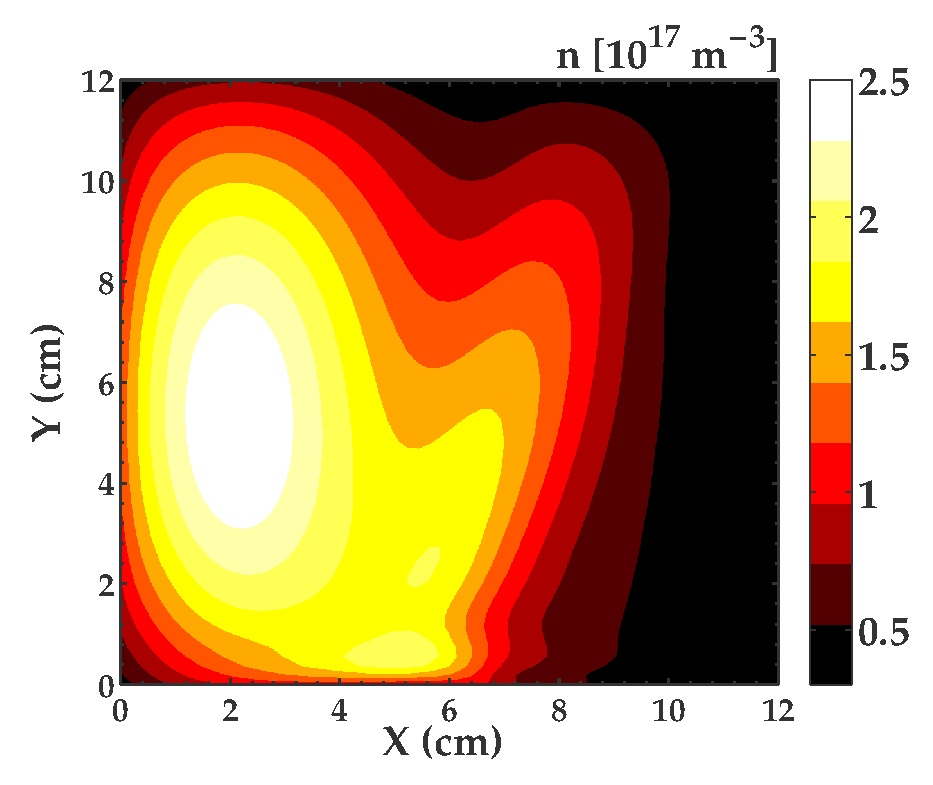
\includegraphics[width=4cm]{figures/4-PegasesCarteDensiteBase.eps}}
    \subfigure[]{\label{4-PegasesCartePotentielBase}
    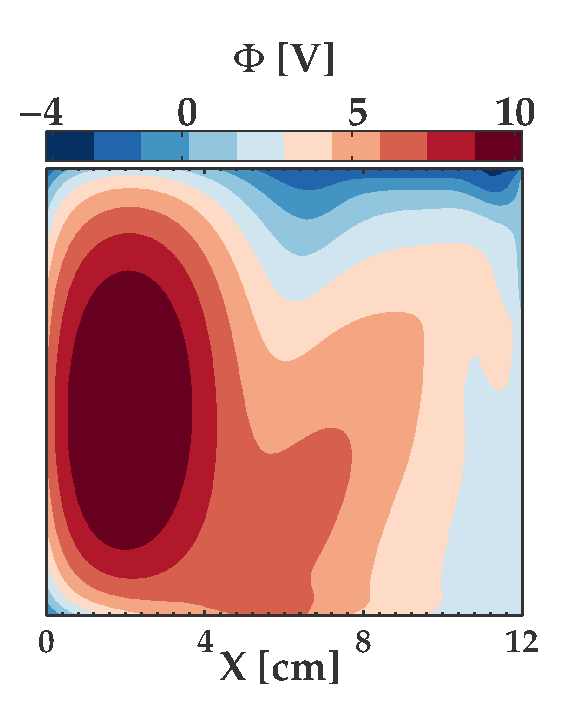
\includegraphics[width=4cm]{figures/4-PegasesCartePotentielBase.eps}}
    \subfigure[]{\label{4-PegasesCarteTemperatureBase}
    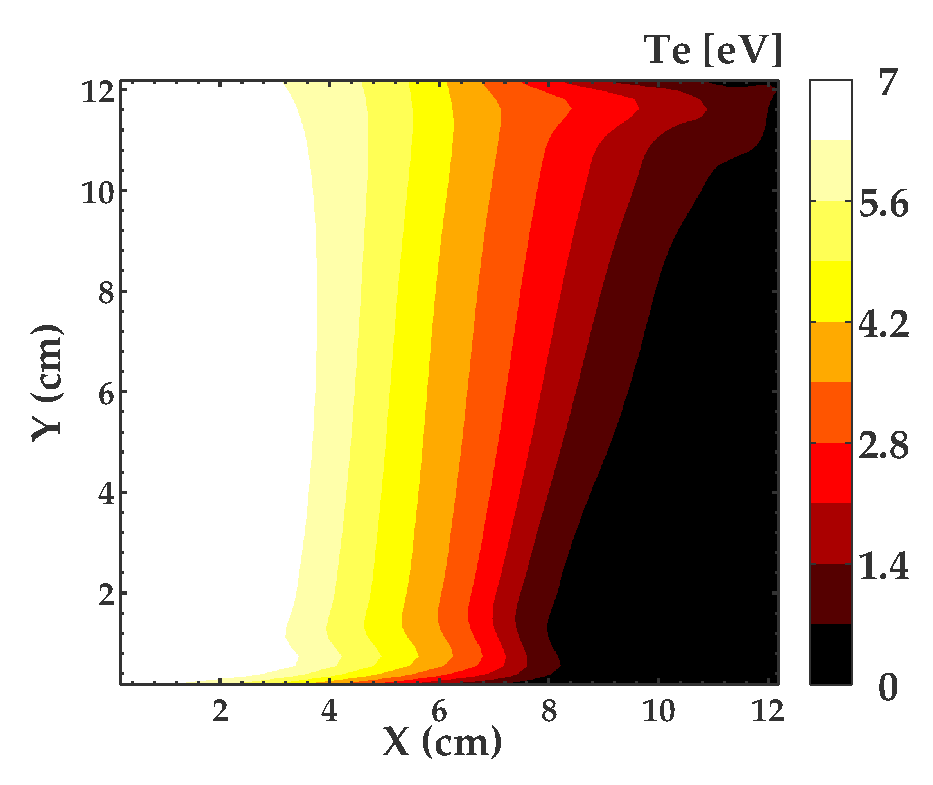
\includegraphics[width=4cm]{figures/4-PegasesCarteTemperatureBase.eps}}
    \caption{Cartes de densité \subref{2-CarteDensiteBase} et de potentiel
    \subref{2-CartePotentielBase}}
    \label{pandas}
\end{figure}

		\subsection{Comparaison expérimentale}
			
			\subsubsection{Variation de l'intensité du champ magnétique}
			\subsubsection{Variation de l'intensité du champ magnétique}


	
	\section{CYBELE Colonne de plasma magnétisé}
		

%\bibliographystyle{apalike}
%\bibliography{biblio}
\end{refsection}
